% Drawing 156-9/01-1 -- folder 156-9, batch 01, archive page 1 (PDF page 2).
% Transcription: un graphe des types d'ateliers, reliés par des traits et des flèches. En haut, « Atelier général $(\mathcal{A};\trianglelefteq,\mathring{\ll},|o|)$ » cerclé ($\mathcal{A}$) ; sous lui « Atelier divisible » (souligné, traversé par le trait qui monte vers l'atelier général). Au niveau suivant : « atelier spatial $(\mathcal{A};\trianglelefteq,|o|)$ » avec $\Sigma$ cerclé, relié à l'atelier général ; « atelier local $(\mathcal{A};\trianglelefteq,\mathring{\ll},|o|_{\mathcal{L}})$ » ; « atelier fidèle $(\mathcal{A};\trianglelefteq,\mathring{\ll})$ », relié à l'atelier général. Plus bas, « atelier ponctuel $\Sigma\simeq\mathfrak{P}(\mathcal{L})$ », relié à l'atelier local et à l'atelier fidèle, et par un trait tireté à l'atelier spatial ; une flèche de l'atelier spatial et une flèche de l'atelier ponctuel descendent vers ($\mathcal{L}$) « atelier ensembliste », d'où une flèche vers « at. ens. modéré », puis vers « at. discret », puis vers « at.-point » (au-dessus, un mot biffé, \ill{}). À droite, « atelier modéré » (un premier « atelier modéré » est biffé plus haut) reçoit une longue courbe venue de l'atelier général et une autre de l'atelier fidèle, avec au crayon « at. mod ? » ; une flèche tiretée en part vers « at. ens. modéré » ; « maquette $\Sigma\simeq\mathfrak{P}(\mathcal{A})$ », encadrée au crayon, est reliée par une double flèche à l'atelier modéré et envoie une flèche vers « at. discret ». Un trait horizontal orangé sépare « at. discret » et « at.-point » du reste.
% Kind: graph of the types of ateliers. Method 2 (schematic redraw from the facsimile). Status: partial.
% Notes: The nodes as on the page, with their formulas as the transcription reads them: atelier général (circled A), atelier divisible (crossed by the stroke up to the general atelier), atelier spatial (circled Sigma), atelier local, atelier fidèle, atelier ponctuel Sigma = P(L), pencil "at. mod ?", (circled L) atelier ensembliste, atelier modéré (an earlier struck "atelier modéré" at the top right), at. ens. modéré, maquette Sigma = P(A) in its pencil box, at. discret, at.-point (a struck word above it); the strokes and arrows between them, dashed where dashed, the double arrow maquette - atelier modéré, and the orange horizontal line. The pencil NB box at the right edge and a few faint pencil strokes are left out; the long curves are approximate.
% Coordinates: 1 unit = 1 mm = 1/100 of the crop width (bbox in page fractions: [0.1, 0.17, 0.8, 0.6]).
% Redrawn by Claude (claude-opus-5-5), issue #73, 2026-11-07; not checked by a human; not compiled (no TeX in the session).
% Rights: reproduces part of the work -- behind RENDER_TRANSCRIPTS, never published by itself.
\documentclass[tikz,border=3pt]{standalone}
\usepackage{amsmath,amssymb}
\usetikzlibrary{patterns,arrows.meta}
\tikzset{Or/.style={orange!90!black}, pencil/.style={black!45}, struck/.style={black!35}, mark/.style={circle,draw,inner sep=1.3pt}, pt/.style={circle,fill,inner sep=0.9pt}, opt/.style={circle,draw,fill=white,inner sep=1.1pt}}
\begin{document}
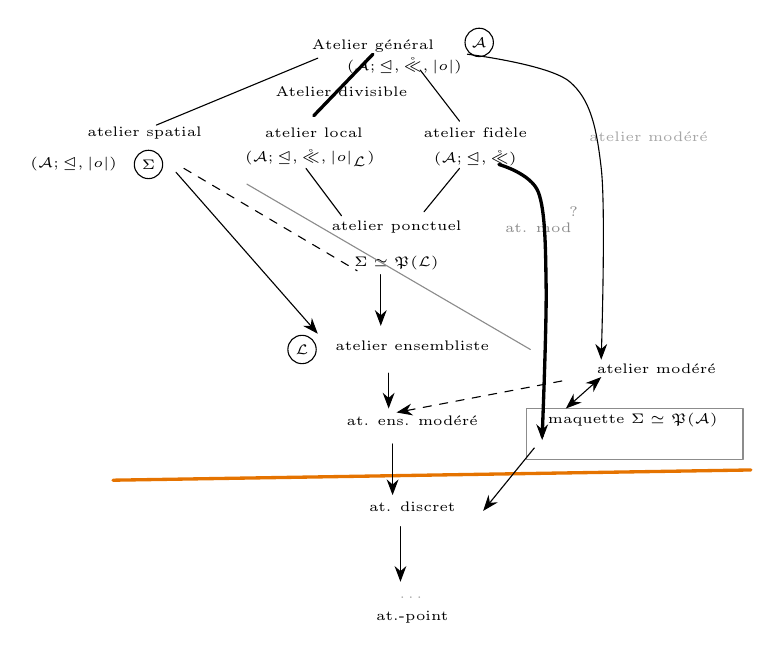
\begin{tikzpicture}[x=1mm,y=1mm,line cap=round,line join=round,font=\scriptsize]
\node[inner sep=1pt] at (52,-9.5) {\tiny Atelier général};
\node[inner sep=1pt] at (56,-12) {\tiny $(\mathcal A;\trianglelefteq,\mathring{\ll},|o|)$};
\draw (65.5,-9) circle[radius=1.8];
\node[inner sep=1pt] at (65.5,-9) {\tiny $\mathcal A$};
\node[inner sep=1pt] at (48,-15.3) {\tiny Atelier divisible};
\draw[very thick] (44.5,-18.3) -- (52,-10.5);
\node[inner sep=1pt] at (23,-20.5) {\tiny atelier spatial};
\node[inner sep=1pt] at (14,-24.5) {\tiny $(\mathcal A;\trianglelefteq,|o|)$};
\draw (23.5,-24.5) circle[radius=1.8];
\node[inner sep=1pt] at (23.5,-24.5) {\tiny $\Sigma$};
\node[inner sep=1pt] at (44.5,-20.5) {\tiny atelier local};
\node[inner sep=1pt] at (44,-23.7) {\tiny $(\mathcal A;\trianglelefteq,\mathring{\ll},|o|_{\mathcal L})$};
\node[inner sep=1pt] at (65,-20.5) {\tiny atelier fidèle};
\node[inner sep=1pt] at (65,-23.7) {\tiny $(\mathcal A;\trianglelefteq,\mathring{\ll})$};
\node[inner sep=1pt,struck] at (87,-21) {\tiny atelier modéré};
\node[inner sep=1pt] at (55,-32.5) {\tiny atelier ponctuel};
\node[inner sep=1pt] at (55,-37) {\tiny $\Sigma\simeq\mathfrak P(\mathcal L)$};
\node[inner sep=1pt,pencil] at (73,-32.5) {\tiny at. mod};
\node[inner sep=1pt,pencil] at (77.5,-30.5) {\tiny ?};
\draw (43,-48) circle[radius=1.8];
\node[inner sep=1pt] at (43,-48) {\tiny $\mathcal L$};
\node[inner sep=1pt] at (57,-47.5) {\tiny atelier ensembliste};
\node[inner sep=1pt] at (88,-50.5) {\tiny atelier modéré};
\node[inner sep=1pt] at (57,-57) {\tiny at. ens. modéré};
\node[inner sep=1pt] at (85,-57) {\tiny maquette $\Sigma\simeq\mathfrak P(\mathcal A)$};
\draw[pencil] (71.5,-55.5) -- (99,-55.5) -- (99,-62) -- (71.5,-62) -- cycle;
\draw[Or,very thick] (19,-64.6) -- (100,-63.3);
\node[inner sep=1pt] at (57,-68) {\tiny at. discret};
\node[inner sep=1pt,struck] at (57,-79.5) {\tiny \ldots};
\node[inner sep=1pt] at (57,-82) {\tiny at.-point};
\draw (24.5,-19.5) -- (45,-11);
\draw (63,-19) -- (58,-12.5);
\draw plot[smooth, tension=0.55] coordinates {(64,-10.5) (77,-14) (81,-25) (81,-49)};
\draw[-{Stealth[length=2mm]}] (81,-47) -- (81,-49.3);
\draw[very thick] plot[smooth, tension=0.55] coordinates {(68,-24.5) (73,-28) (74,-40) (73.5,-59)};
\draw[-{Stealth[length=2mm]}] (73.5,-57) -- (73.5,-59.5);
\draw (43.5,-25) -- (48,-31);
\draw (63,-25) -- (58.5,-30.5);
\draw[dashed] (28,-25) -- (50,-38);
\draw[-{Stealth[length=2mm]}] (27,-25.5) -- (45,-46);
\draw[pencil] (36,-27) -- (72,-48);
\draw[-{Stealth[length=2mm]}] (53,-38.5) -- (53,-45);
\draw[-{Stealth[length=2mm]}] (54,-51) -- (54,-55.5);
\draw[-{Stealth[length=2mm]},dashed] (76,-52) -- (55,-56);
\draw[{Stealth[length=2mm]}-{Stealth[length=2mm]}] (76.5,-55.5) -- (81,-51.5);
\draw[-{Stealth[length=2mm]}] (72.5,-60.5) -- (66,-68.5);
\draw[-{Stealth[length=2mm]}] (54.5,-60) -- (54.5,-66.5);
\draw[-{Stealth[length=2mm]}] (55.5,-70.5) -- (55.5,-77.5);
\end{tikzpicture}
\end{document}
